\chapter{after effects} 
\label{sec:patterns}
\rhead[]{\leftmark}
\lstset{style=6502Style}
\lstset{ 
   aboveskip=5pt,
   belowskip=0pt,
}
After Psychedelia, Jeff Minter spent the rest of his working life make 'light synthesizers' of one sort or another. We will cover the very next incarnation of the
Psychedelia concept in our companion volume 'Colourspace Complex', an exploration of the 1985 title 'Colourspace' written just a few months after the C64 original
which took advantage of the superior graphical capabilities and colour palette of the Atari 800. 

But Minter himself didn't stop with the Atari 800. He went on to develop the light
synthesiser concept on nearly every generation of video game console released
over the next thirty years. Some of these efforts were doomed by the failure of
the platform they were written for, such as the 'Virtual Light Machine' on the
ill-fated Atari Jaguar and the 'VLM 1' for the now rapidly defunct Nuon DVD platform developed by
VM Labs. This chequered history culminated in something of a small triumph, when his PC-generation version of the Virtual Light Machine engine, known as 'Neon',
was incorporated into the XBOX 360 when it was released in 2005. For the first time in his career, Minter's light synthesizer went mainstream and was put in the
hands of millions of customers.

For us though, we will end in 1985, with Minter's final iteration of his light machine on 8-bit hardware: a psychedelic sub-game in his 1985 title 'Batalyx'. Here
we find the idea reduced again to its kernel, back to a version of its beginnings in PC Computer Weekly magazine as a short lump of code that can fit on a few pages.
Like the listing we acquainted ourselves at the start of this book, the version of Psychedelia in 'Batalyx' supports only a single lightform (or pattern) and only
minimal configuration. Minter's motivation was simple:

\subfile{after_effects/batalyx_listing.tex}

\begin{figure}[H]
    \centering
    \begin{adjustbox}{width=11cm,center}
      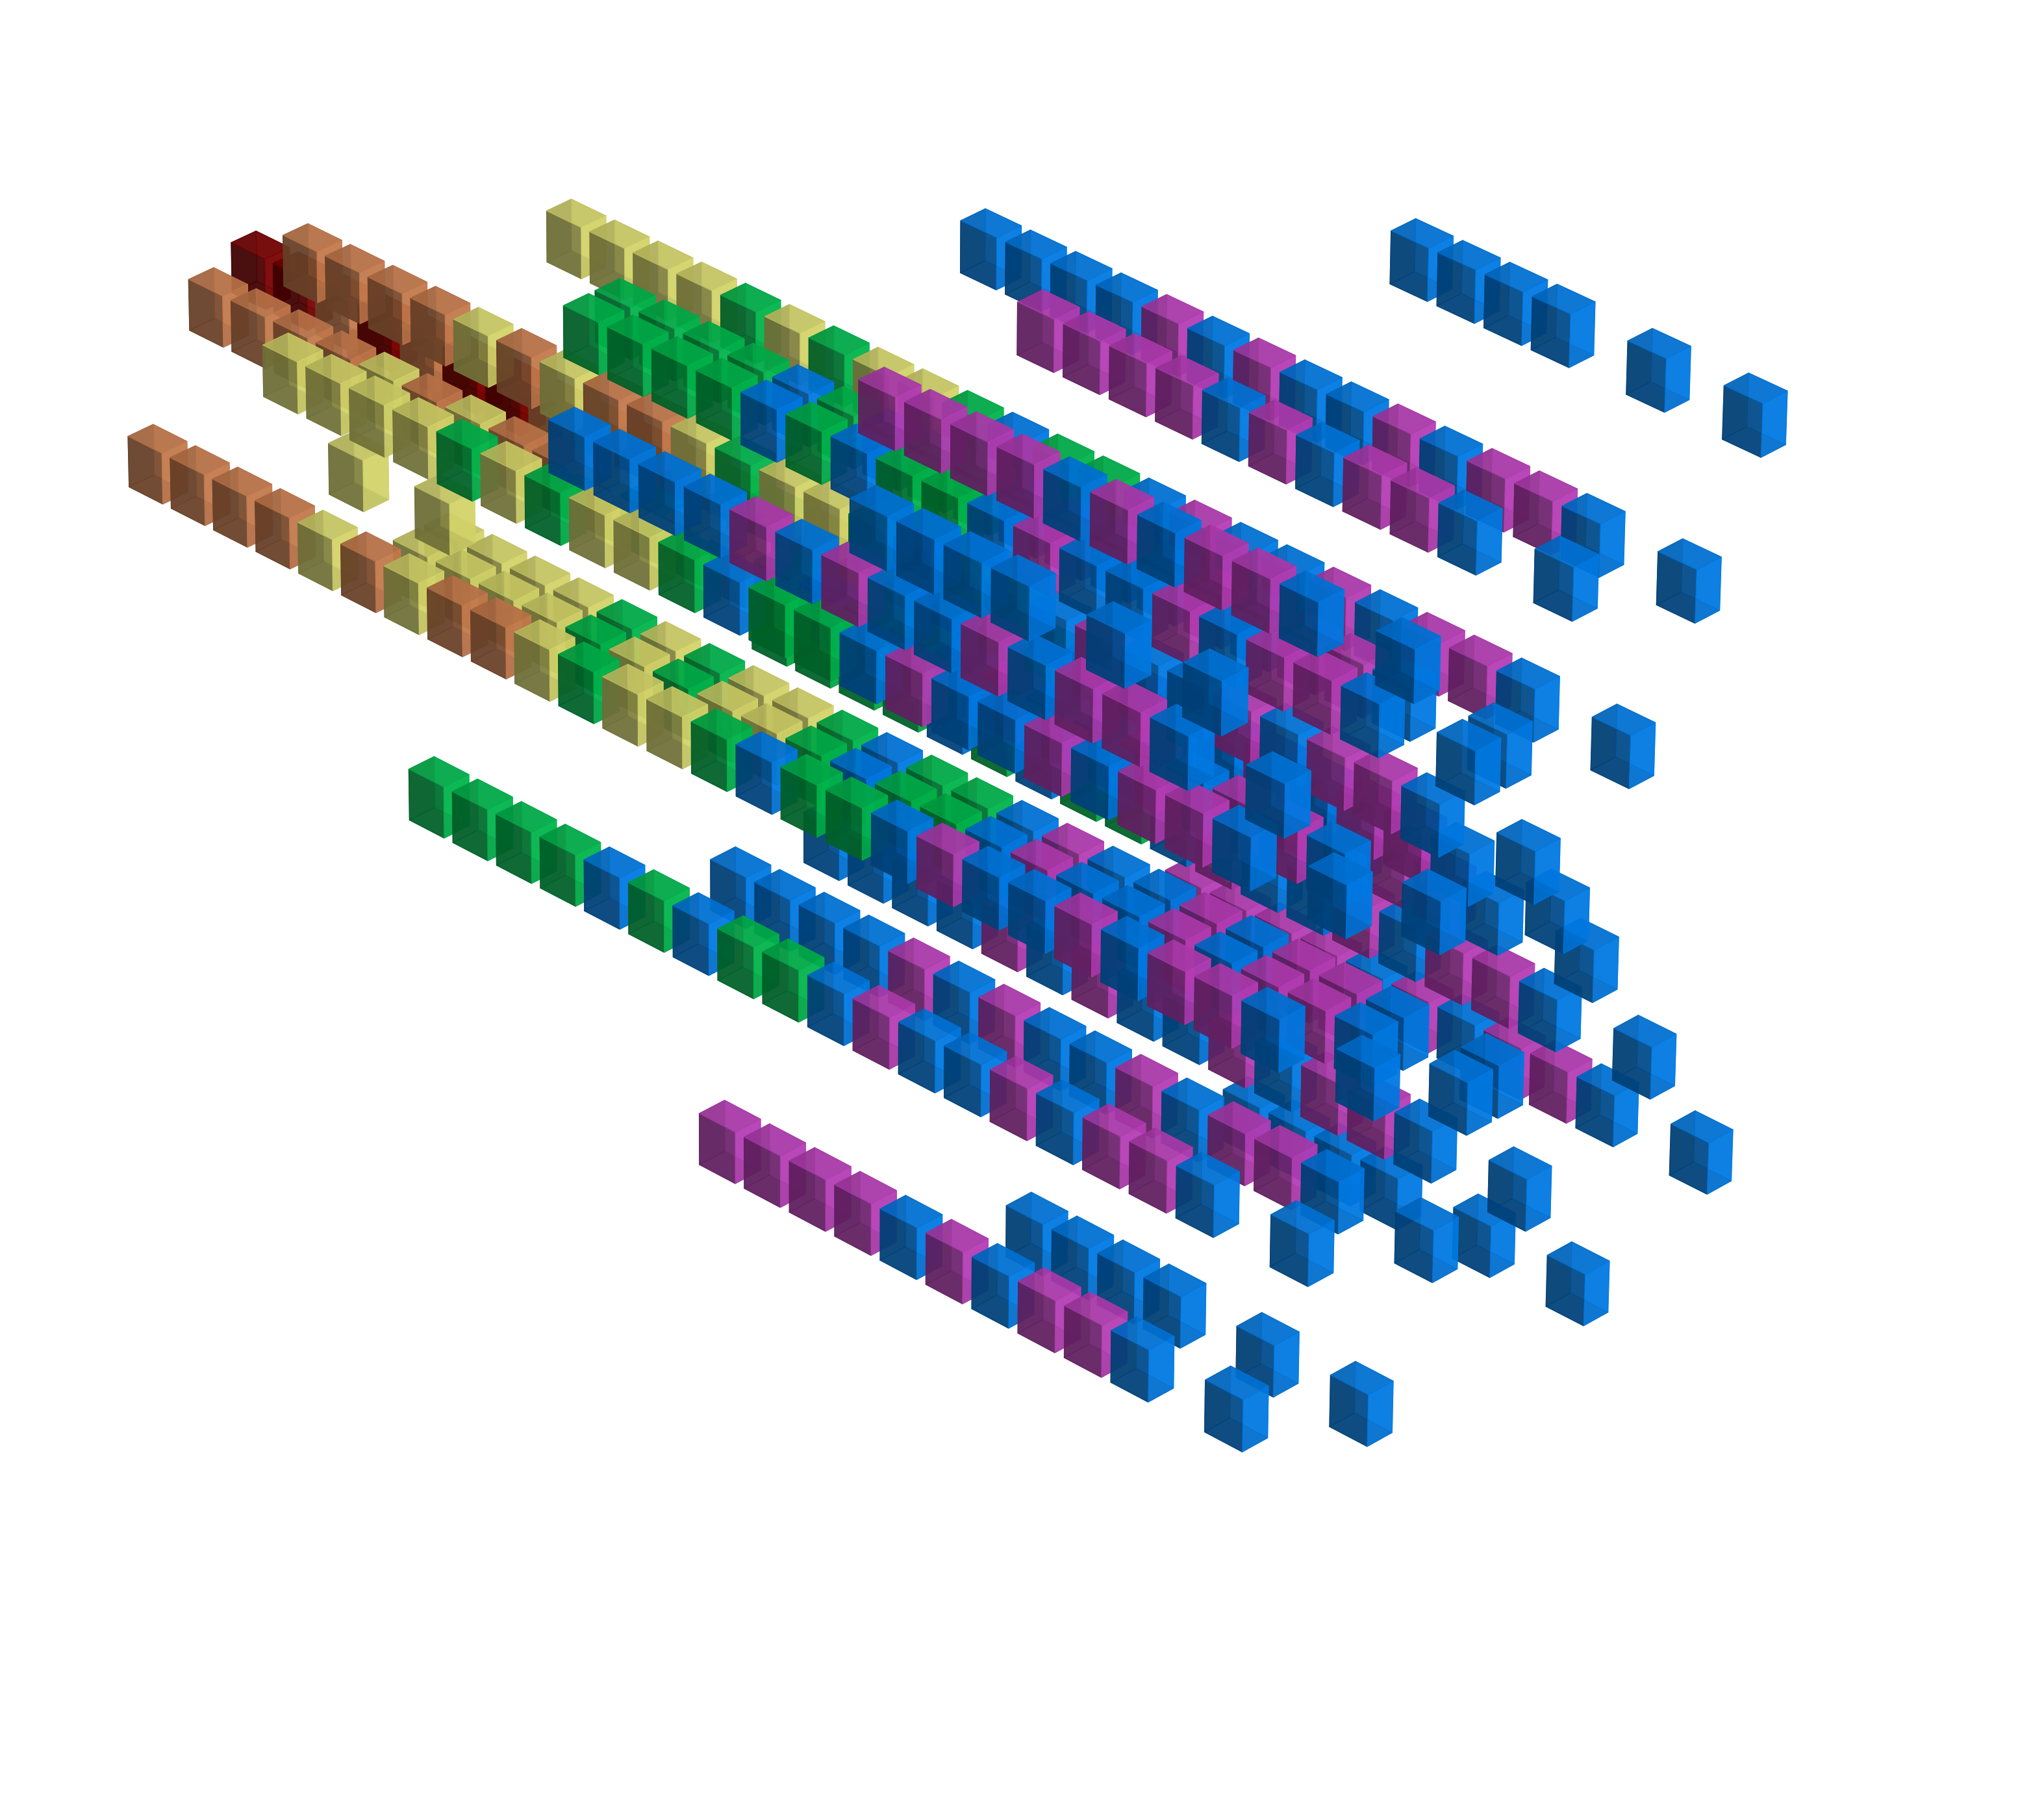
\includegraphics[width=11cm]{src/batalyx_patterns/pattern0-45.png}%
    \end{adjustbox}
    \begin{adjustbox}{width=11cm,margin=0cm -2cm}
      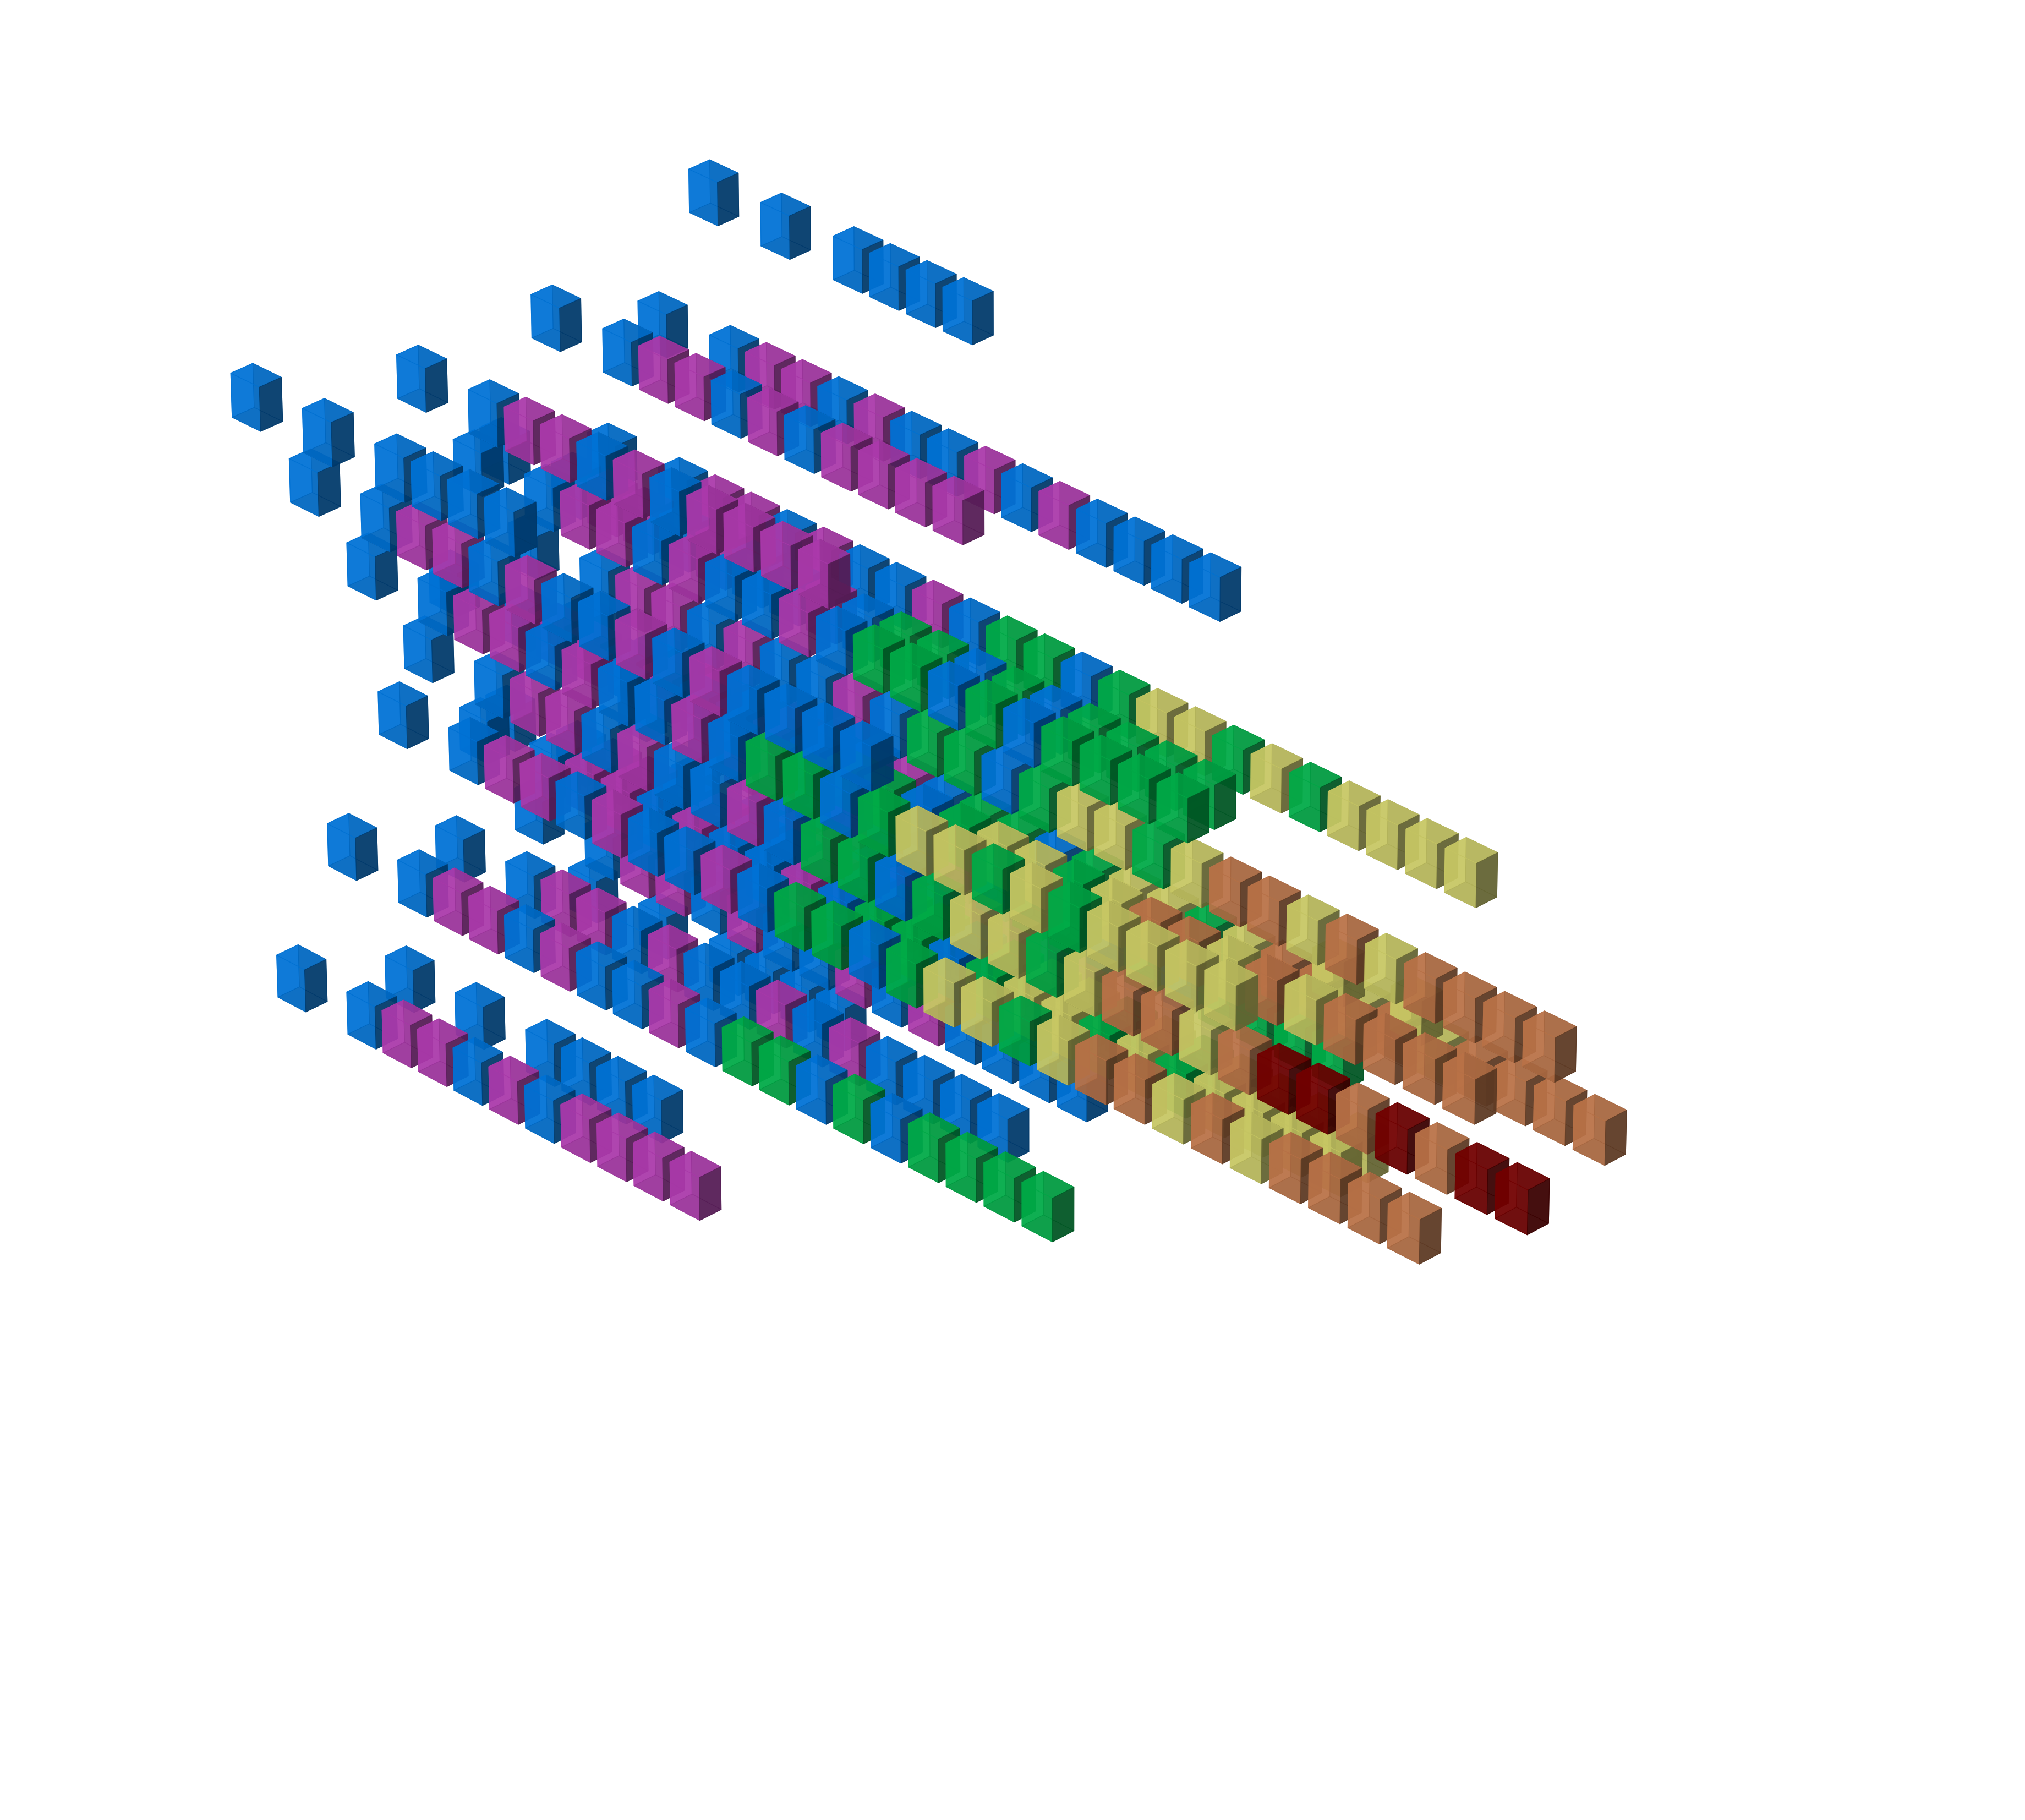
\includegraphics[width=11cm]{src/batalyx_patterns/pattern0-225.png}%
    \end{adjustbox}
\caption{Evolution of the 'Batalyx' pattern.}
\end{figure}

\rhead[]{Star One}
\begin{lstlisting}[caption=Source code for the Batalyx pattern..]
patternXPosArray             
        .BYTE $FF,$01,$55    ; 6              
        .BYTE $FE,$02,$55    ;            5   
        .BYTE $FD,$03,$55    ;   4            
        .BYTE $FC,$04,$55    ;          3     
        .BYTE $FB,$05,$55    ;     2          
        .BYTE $FA,$06,$55    ;        1       
        .BYTE $55,$55        ;                
patternYPosArray             ;      1         
        .BYTE $01,$FF,$55    ;         2      
        .BYTE $FE,$02,$55    ;    3           
        .BYTE $03,$FD,$55    ;           4    
        .BYTE $FC,$04,$55    ;  5             
        .BYTE $05,$FB,$55    ;             6 
        .BYTE $FA,$06,$55
        .BYTE $55,$55
\end{lstlisting}

\subfile{batalyx_patterns/tables/pattern0.tex}

\clearpage
\textbf{Lines 1189-1231. \icode{\textbf{LaunchPsychedelia}}} 
\begin{lstlisting}
;--------------------------------------------------------
; LaunchPsychedelia
;--------------------------------------------------------
LaunchPsychedelia
        SEI 
        JSR InitializePsychedelia
        JSR SetUpBackgroundPainting
        JSR InitializeColorIndexArray
        JSR InitializeStatusDisplayText
        JSR UpdateCurrentSettingsDisplay
        CLI 
PsychedeliaLoop   
        JSR MaybeUpdateFromBuffersAndPaint
        JSR CheckKeyboardInput
        JMP PsychedeliaLoop
\end{lstlisting}
\textbf{Lines 1189-1231. \icode{\textbf{MaybeUpdateFromBuffersAndPaint}}} 
\begin{lstlisting}[basicstyle=\ttfamily\scriptsize, caption=The routine responsible for painting patterns.]
MaybeUpdateFromBuffersAndPaint   
        LDX lastIndexToBuffers
        LDA currentColorIndexArray,X
        AND #$08
        BNE BufferUpdateComplete

        DEC smoothingDelayArray,X
        BNE BufferUpdateComplete

        LDA initialSmoothingDelayArray,X
        STA smoothingDelayArray,X

        LDA pixelXPositionArray,X
        STA currentPixelXPosition
        LDA pixelYPositionArray,X
        STA currentPixelYPosition

        LDA currentColorIndexArray,X
        STA currentColorIndex

        TAY 
        LDA symmetrySettingForStep,X
        STA currentSymmetrySettingForStep

        LDA presetColorValuesArray,Y
        STA currentColor

        INC currentColorIndexArray,X
        JSR PaintStructureAtCurrentPosition

BufferUpdateComplete   
        INC lastIndexToBuffers

        LDA lastIndexToBuffers
        AND #$3F
        STA lastIndexToBuffers
        RTS 
\end{lstlisting}
\clearpage

\rhead[]{\icode{LaunchPsychedelia}}
\textbf{Lines 1189-1231. \icode{\textbf{LaunchPsychedelia}}:} A nice compact launch routine compared to what we're used to. As an added
bonus it also contains the game's main loop in \icode{PsychedeliaLoop}! The first thing to note here is that, unlike all the previous
versions we've looked at, this main loop is also checking keyboard input - something previously managed by the interrupt handler. The
interrupt handler, as well as animating the background, still looks after joystick input but the reduced set of keyboard commands and
the increased load on the interrupt handler, means that we can fit the keyboard check in here instead.

\bigskip
\bigskip
\bigskip
\bigskip
\bigskip
\textbf{Lines 1189-1231. \icode{\textbf{MaybeUpdateFromBuffersAndPaint}}:} The business end of the main loop which co-ordinates all pattern
painting.


\clearpage
Text fdjsklfdsjklfdsjkfldsjfdskl
\vfill
\begin{figure}[H]                                                          
  \centering                                                             
  \begin{adjustbox}{width=13cm,center}                                   
  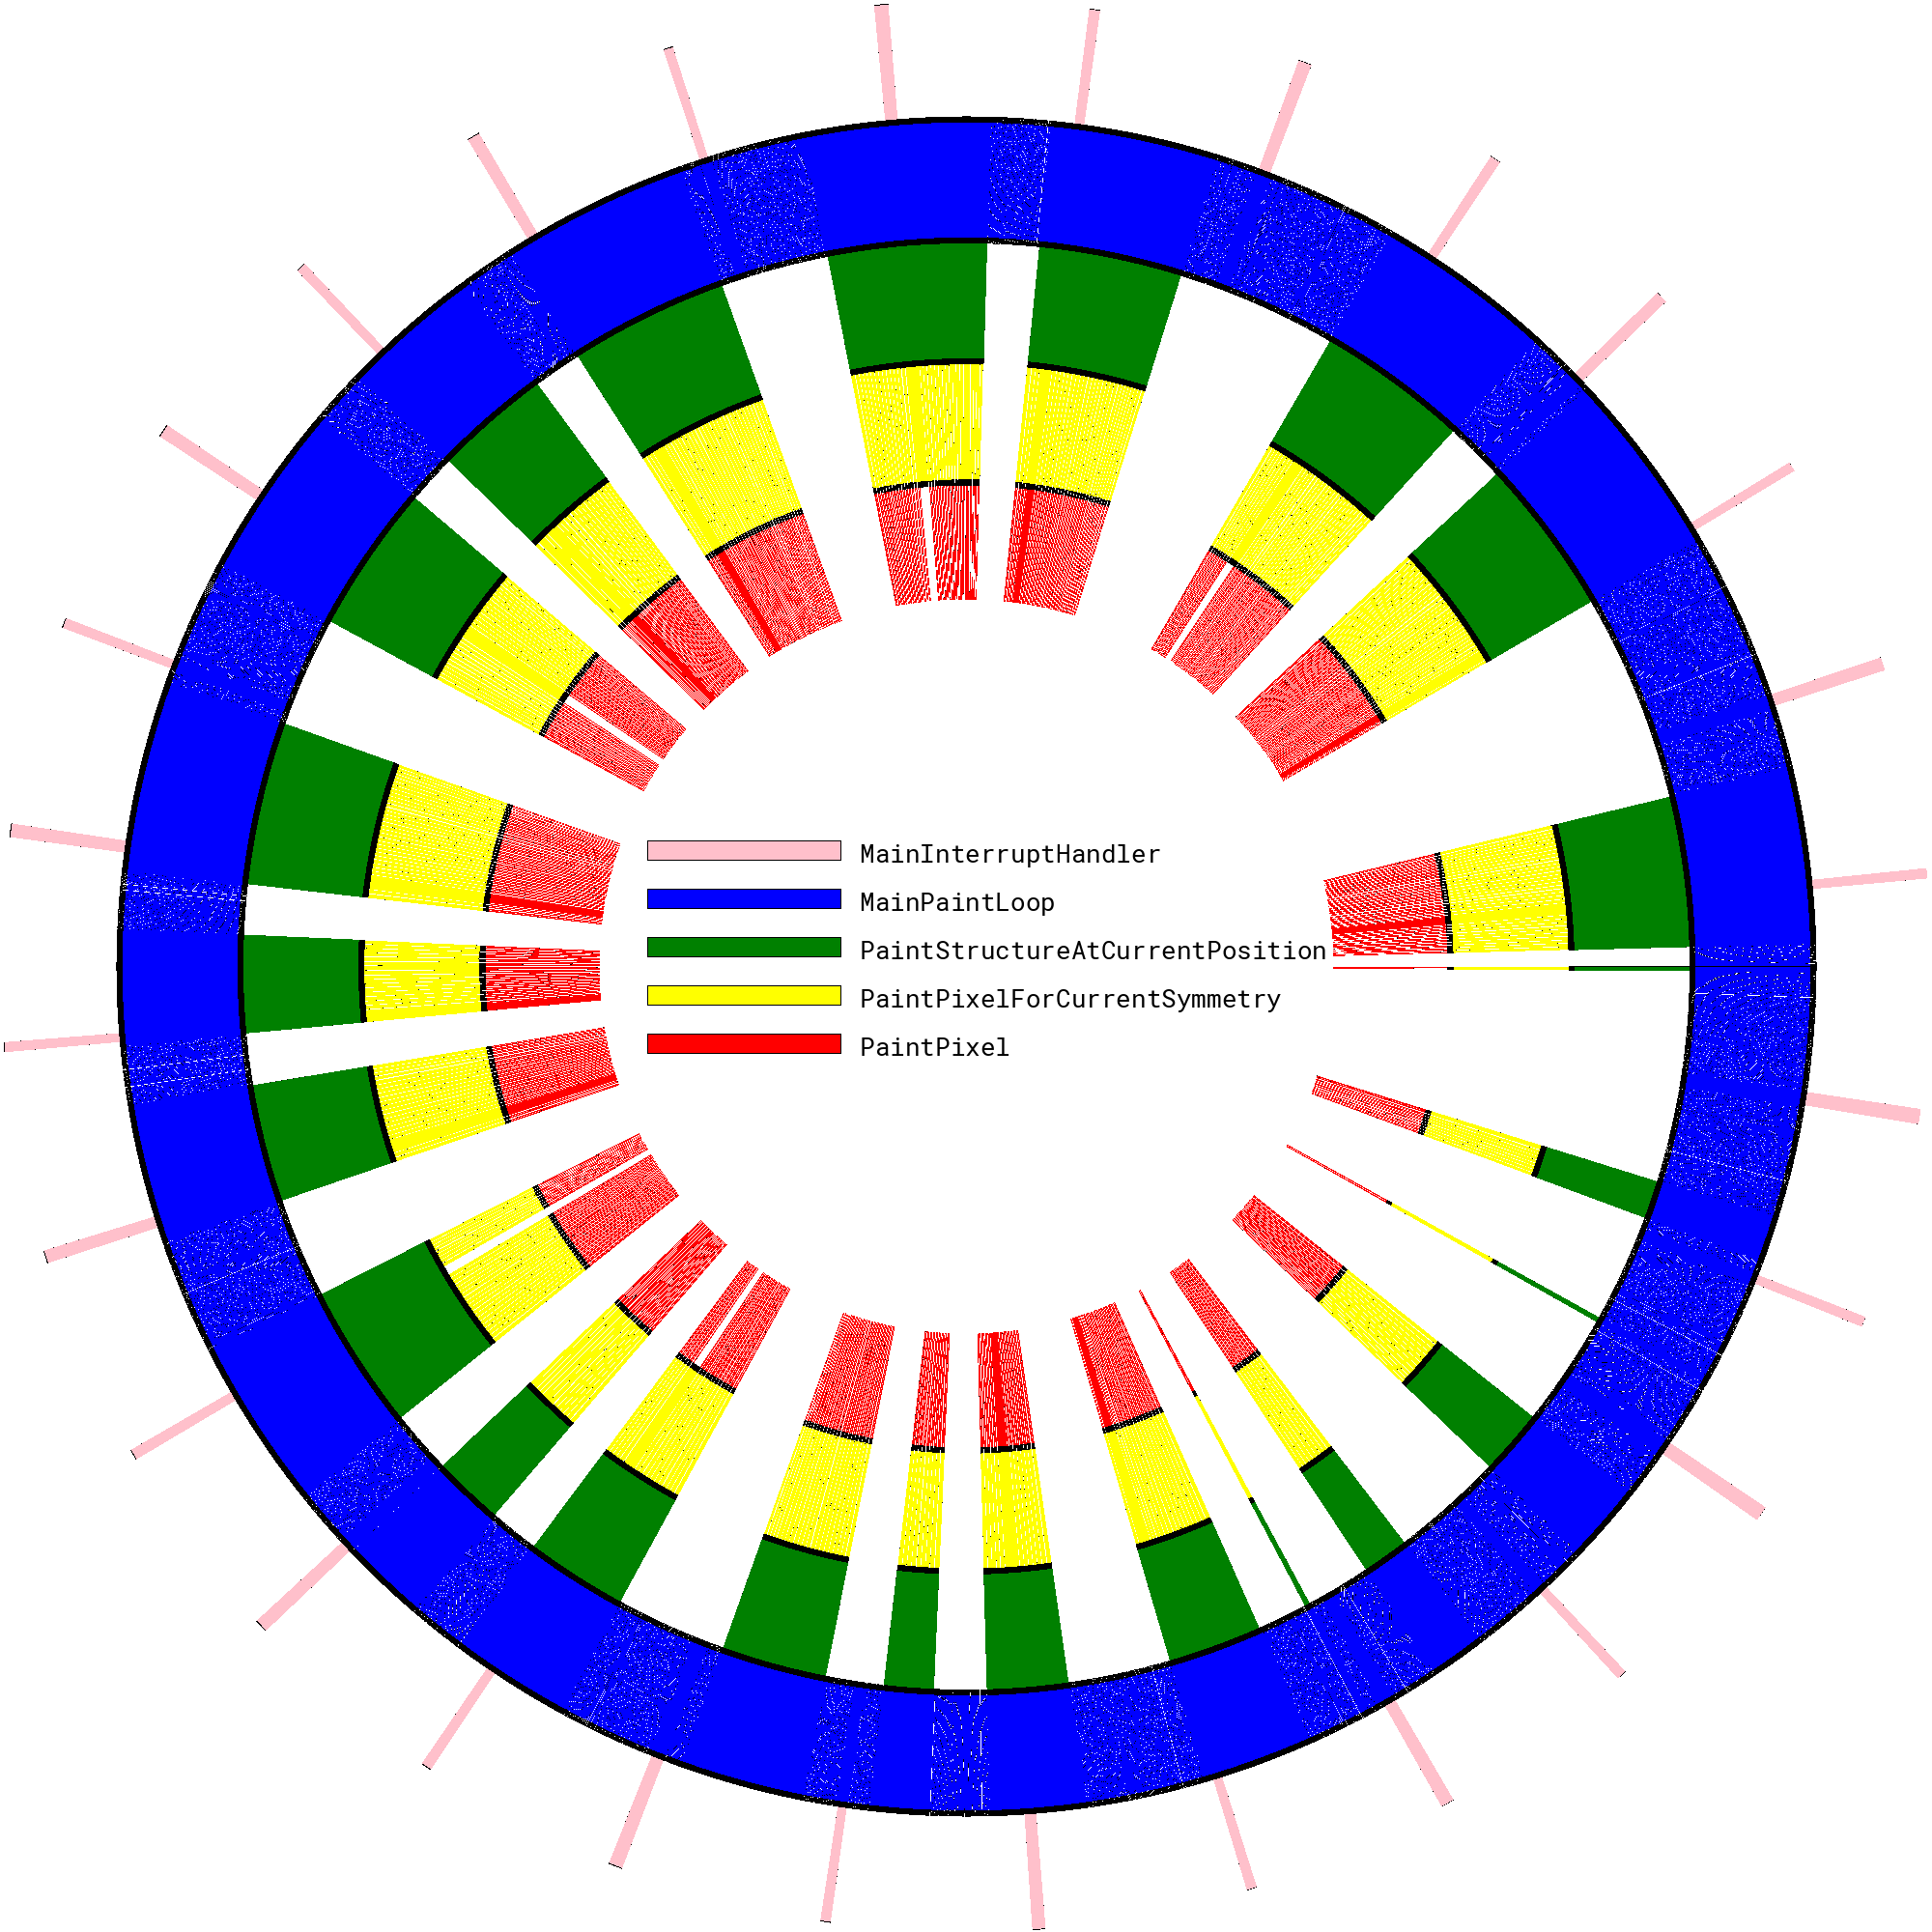
\includegraphics[width=13cm]{src/listing_commentary/execution_cycle.png}%           
  \end{adjustbox}                                                        
\caption{The execution map of a full pattern evolution in the original edition of Psychedelia.}                                           
\end{figure}                                                               
\vfill
\clearpage
Text fdjsklfdsjklfdsjkfldsjfdskl
\vfill
\begin{figure}[H]                                                          
  \centering                                                             
  \begin{adjustbox}{width=13cm,center}                                   
  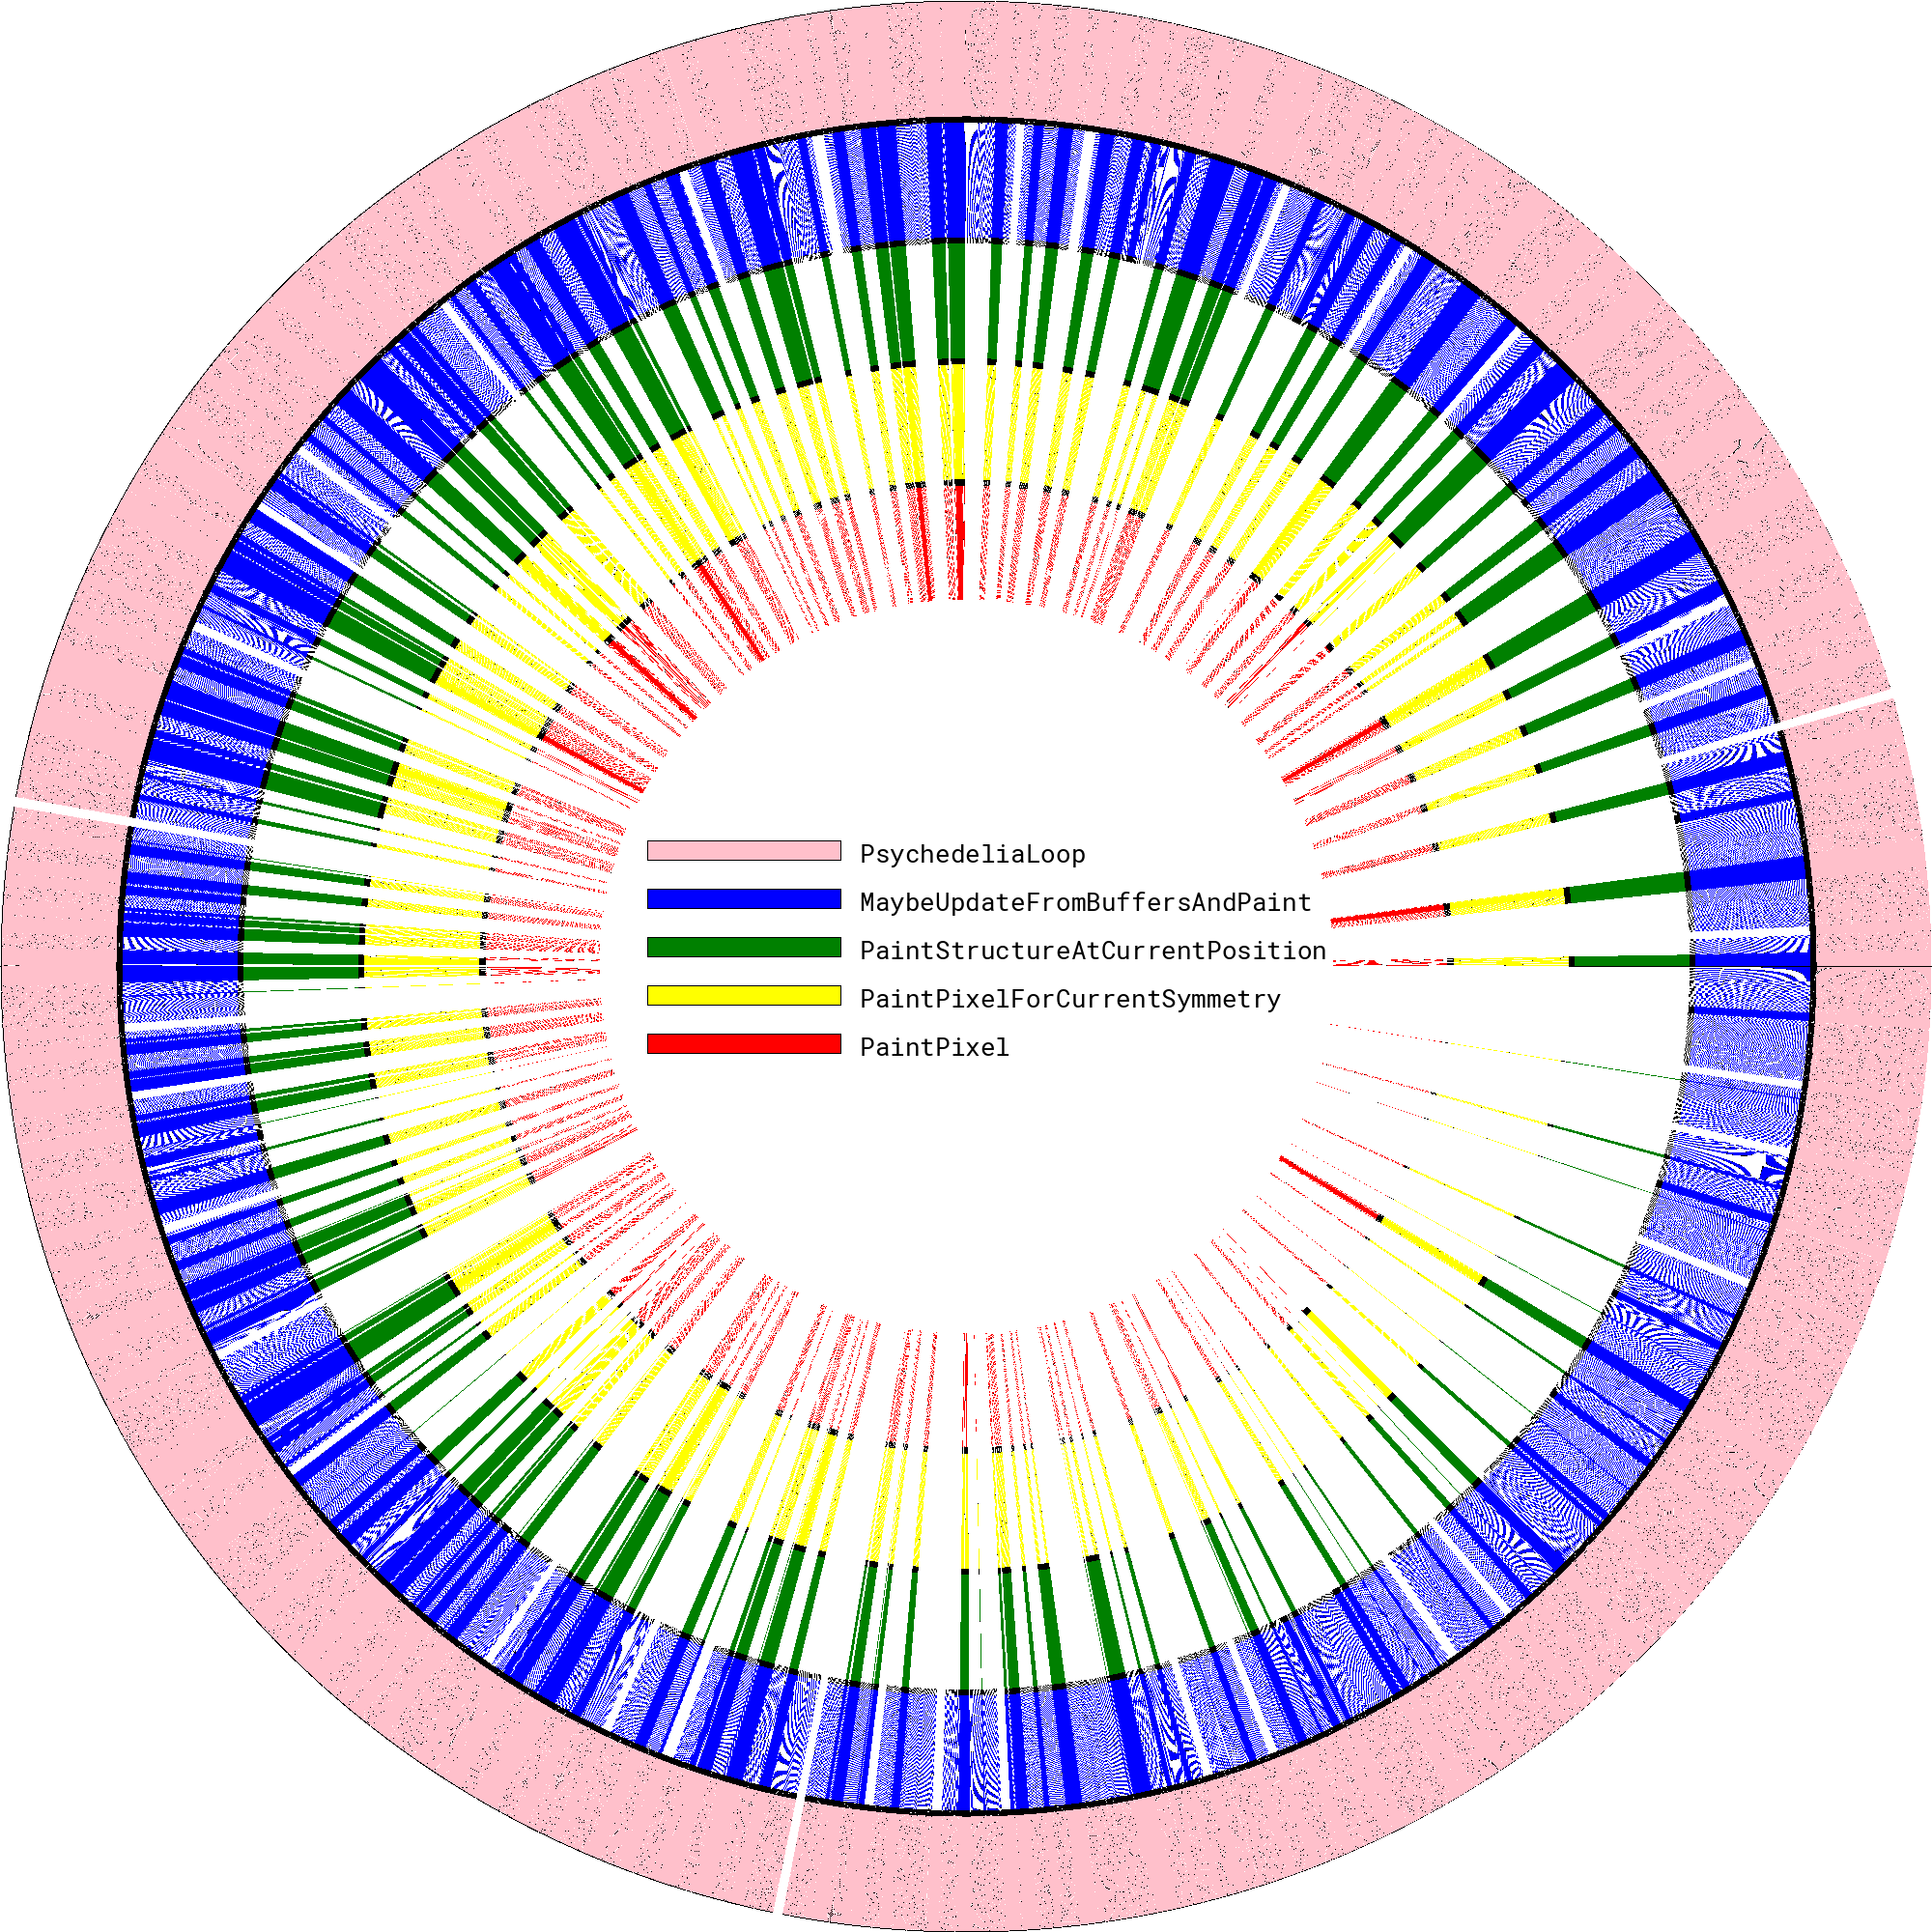
\includegraphics[width=13cm]{src/after_effects/execution_cycle.png}%           
  \end{adjustbox}                                                        
\caption{The execution map of a full pattern evolution in the Batalyx edition of Psychedelia.}                                           
\end{figure}                                                               
\vfill

\clearpage
\textbf{Lines 1189-1231. \icode{\textbf{PaintStructureAtCurrentPosition}}} 
\begin{lstlisting}[caption = All the pattern data structures in Psychedelia organized into a set of arrays.]
;--------------------------------------------------------
; PaintStructureAtCurrentPosition
;--------------------------------------------------------
PaintStructureAtCurrentPosition   
        LDA #$00
        STA currentPatternIndex
        STA currentLineInPattern

        LDA currentPixelXPosition
        STA initialPixelXPosition
        LDA currentPixelYPosition
        STA initialPixelYPosition

        JSR PaintPixelForCurrentSymmetry

        LDA currentColorIndex
        BNE PixelPaintLoop
        RTS 

PixelPaintLoop   
        LDX currentPatternIndex
        LDA patternXPosArray,X
        CMP #$55
        BEQ MoveToNextLineInPattern

        CLC 
        ADC currentPixelXPosition
        STA initialPixelXPosition

        LDA patternYPosArray,X
        CLC 
        ADC currentPixelYPosition
        STA initialPixelYPosition

        JSR PaintPixelForCurrentSymmetry

        INC currentPatternIndex
        JMP PixelPaintLoop

MoveToNextLineInPattern   
        INC currentPatternIndex
        INC currentLineInPattern
        LDA currentLineInPattern
        CMP currentColorIndex
        BNE PixelPaintLoop
        RTS 
\end{lstlisting}
\clearpage

\rhead[]{\icode{PaintStructureAtCurrentPosition}}
\textbf{Lines 1189-1231. \icode{\textbf{PaintStructureAtCurrentPosition}}:} Psychedelia

\clearpage
\textbf{Lines 1189-1231. \icode{\textbf{PaintPixelForCurrentSymmetry}}} 
\begin{lstlisting}[basicstyle=\ttfamily\scriptsize, caption=The routine responsible for painting patterns.]
;--------------------------------------------------------
; PaintPixelForCurrentSymmetry
;--------------------------------------------------------
PaintPixelForCurrentSymmetry   
        LDA initialPixelYPosition
        AND #$80
        BEQ CanPaintPixelOnThisLine

CleanUpAndReturn   
        RTS 

CanPaintPixelOnThisLine   
        LDA initialPixelYPosition
        CMP #TOP_Y_POSITION+1
        BPL CleanUpAndReturn

        LDA initialPixelXPosition
        AND #$80
        BNE CleanUpAndReturn

        LDA initialPixelXPosition
        CMP #NUM_COLS
        BPL CleanUpAndReturn

        LDA currentColor
        TAX 
        LDA colorComparisonArray,X
        STA lastColorValue
        DEC lastColorValue

        JSR PaintPixel

        LDA currentSymmetrySettingForStep
        BNE HasSymmetry

ReturnFromSymmetry   
        RTS 

\end{lstlisting}
\clearpage

\rhead[]{\icode{LaunchPsychedelia}}
\textbf{Lines 1189-1231. \icode{\textbf{LaunchPsychedelia}}:} A nice compact launch routine compared to what we're used to. As an added
bonus it also contains the game's main loop in \icode{PsychedeliaLoop}! The first thing to note here is that, unlike all the previous
versions we've looked at, this main loop is also checking keyboard input - something previously managed by the interrupt handler. The
interrupt handler, as well as animating the background, still looks after joystick input but the reduced set of keyboard commands and
the increased load on the interrupt handler, means that we can fit the keyboard check in here instead.

\textbf{Lines 1189-1231. \icode{\textbf{MaybeUpdateFromBuffersAndPaint}}:} The business end of the main loop which co-ordinates all pattern
painting.

\clearpage
\textbf{Lines 1189-1231. \icode{\textbf{PaintPixelForCurrentSymmetry} continued.}} 
\begin{lstlisting}[caption = All the pattern data structures in Psychedelia organized into a set of arrays.]
HasSymmetry   
        CMP #X_Y_SYMMETRY
        BEQ HasXYSymmetry

        CMP #X_AXIS_SYMMETRY
        BEQ HasXAxisSymmetry

        LDA #NUM_COLS-1
        SEC 
        SBC initialPixelXPosition
        STA initialPixelXPosition

        JSR PaintPixel

        LDA currentSymmetrySettingForStep
        CMP #Y_AXIS_SYMMETRY
        BEQ ReturnFromSymmetry

        LDA #TOP_Y_POSITION
        SEC 
        SBC initialPixelYPosition
        STA initialPixelYPosition

        JSR PaintPixel

        LDA #NUM_COLS-1
        SEC 
        SBC initialPixelXPosition
        STA initialPixelXPosition

        JMP PaintPixel

HasXYSymmetry   
        LDA #TOP_Y_POSITION
        SEC 
        SBC initialPixelYPosition
        STA initialPixelYPosition

        JMP PaintPixel

HasXAxisSymmetry   
        LDA #NUM_COLS-1
        SEC 
        SBC initialPixelXPosition
        STA initialPixelXPosition
        JMP HasXYSymmetry
\end{lstlisting}
\clearpage

\rhead[]{\icode{LaunchPsychedelia}}
\textbf{Lines 1189-1231. \icode{\textbf{LaunchPsychedelia}}:} Psychedelia
\clearpage
\textbf{Lines 1189-1231. \icode{\textbf{PaintPixel}}} 
\begin{lstlisting}[caption = All the pattern data structures in Psychedelia organized into a set of arrays.]
;--------------------------------------------------------
; PaintPixel
;--------------------------------------------------------
PaintPixel   
        LDX initialPixelYPosition
        LDY initialPixelXPosition
        LDA screenLinesLoPtrArray,X
        STA colorRAMLoPtr
        LDA screenLinesHiPtrArray,X
        CLC 
        ADC #OFFSET_TO_COLOR_RAM
        STA colorRAMHiPtr
        LDA (colorRAMLoPtr),Y
        AND #$0F
        CMP currentColorValue
        BEQ ActuallyPaintPixel

        TAX 
        LDA colorComparisonArray,X
        CMP lastColorValue
        BEQ ActuallyPaintPixel
        BPL ActuallyPaintPixel
        RTS 

ActuallyPaintPixel   
        LDA currentColor
        STA (colorRAMLoPtr),Y
        RTS 

colorComparisonArray   
        .BYTE ORANGE,ORANGE,WHITE,ORANGE,BLUE,PURPLE,YELLOW,CYAN
        .BYTE RED,ORANGE,ORANGE,ORANGE,ORANGE,ORANGE,GREEN,ORANGE
        .BYTE ORANGE

\end{lstlisting}
\clearpage

\rhead[]{\icode{LaunchPsychedelia}}
\textbf{Lines 1189-1231. \icode{\textbf{LaunchPsychedelia}}:} Psychedelia
\clearpage

\vspace*{\fill}
\begin{figure}[H]
    \centering
      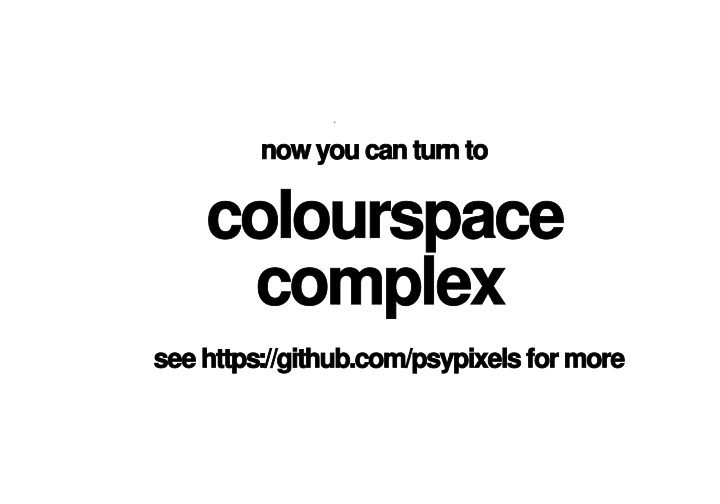
\includegraphics[width=10cm]{src/cover/title_page_colorspace_coming_soon.png}%
\end{figure}

\vspace*{\fill}
